\documentclass[11pt]{jsarticle}

\usepackage{SPR}

\headerSPR
\begin{document}
	\titleSPR{\number\year}{\number\month}{\number\day}{D2}{吉田 皓太郎}
%%%%%%%%%%%%%%%%%%%%%%%%%%%%%%%%%%%%%%
	\articleSPRabst
		\begin{itemize}
			\item 機械学習を用いたカップ形状の設計支援
			\item 着後形状予測のためのカップの変形解析
		\end{itemize}
		
		
	\articleSPRobj
		\begin{enumerate}
			\item 定性的な機能要求を満たせるようなカップ形状を設計できる
			\item 布の物性とカップのパターンがどのような結びつきを持っているかを調べることができる.
		\end{enumerate}
%%%%%%%%%%%%%%%%%%%%%%%%%%%%%%%%%%%%%%
% 1.前回からのノルマ
	\articleSPRitemsone
		%\begin{enumerate}
		%	\item A
		%\end{enumerate}
		
		\tableofcontents
		
		
%%%%%%%%%%%%%%%%%%%%%%%%%%%%%%%%%%%%%%
%\begin{itemize}
%	\item 新規手法について
%	\item ISFAアウトライン
%\end{itemize}
%%%%%%%%%%%%%%%%%%%%%%%%%%%%%%%%%%%%%%
% 2.具体的な成果
	\articleSPRitemstwo
	\renewcommand{\labelitemi}{$\blacktriangledown$}
%%%%%%%%%%%%%%%%%%%%%%%%%%%%%%%%%%%%%%
	\section{投稿論文について}
		修正お願いします.
		
	\section{研究進捗について}
		\subsection{機械学習を用いた機能の定式化などについて}
			今はデータ作成中(なんだかんだ500点近くはデータを生成できるかと・・・).機械学習自体は正誤はともかく,プログラム自体は比較的容易に作成することは可能であるため,データを取ったタイミングで実行する.しかしながら,そのあとどのように問題を設定するかを決まってないので,(今週でなくても)議論できればと思います.(機械学習自体で機能の定量化を行うだけでは,新規性とインパクトに欠けるため)
			また,機械学習の特徴量についてなのですが,SIIの前刷りで定式化した際,$ E,F,G,L,M,N $が次式らで表されることから,よく論文で書いている$ \omega_{\xi},\omega_{\eta},\omega_{\zeta},\alpha $を特徴量として読み込む方針の方がよいかもしれない.
			\begin{eqnarray}
				E &=& (\alpha'+\lambda)^2 t^2 -2\cos \alpha(\alpha'+\lambda) t + 1,\\
				F &=& -\sin \alpha,\\
				G &=& 1,
			\end{eqnarray}
			
			\begin{eqnarray}
				L &=& -\omega_{\xi}+t\{\lambda(-\omega_{\xi}\cos \alpha + \omega_{\zeta}\sin \alpha)+\omega_{\zeta}'\cos \alpha + \omega_{\xi}'\sin \alpha \},  \\
				M &=& \omega_{\xi}\sin \alpha + \omega_{\zeta} \cos \alpha,  \\
				N &=& 0. 
			\end{eqnarray}
			
		\subsection{FEM解析のものについて}
			先日の研究会にて,岩田先生にきちんとシステムの概形を考えるべきではと頂き,その通りであると感じたため,今回は一度,研究目的等を整理した内容を記します.
			まず,設計における要求として,「丸みを持たせたい」という要求がある.紙模型のモデルから,この着用時にはじめて発現する「丸み」は,以下のようなステップで変換されていくと考えられる.
			\begin{figure}[h!]
				\centering
				
\includegraphics[scale=0.5]{./figure/round.png}
				\caption{丸みと紙模型モデルとの関係性}
			\end{figure}
			まず,アイデアの一つとして,この流れを追っていき,ある丸みの設計評価と紙模型モデル(パターン形状)を定量的に結びつけることである.次に全体のシステムとして,二つのアイデアがある.
			
			一つは,丸みそのものの定量的評価を与えず,あるカップの変位分布がもうすでに与えられている場合において,紙模型の設計がどのように達成されるかを計算するものである.これをフロチャートにて示すと,以下のように示す.
			\begin{figure}[h!]
				\centering
				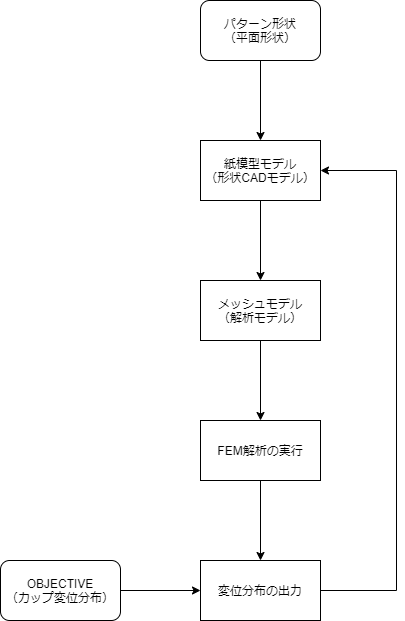
\includegraphics[scale=0.5]{./figure/caseB.png}
				\caption{システムフロチャート1}
			\end{figure}
		
			もう一つは,設計評価が最終的に設計者が確認した際に決定し,ある部分を修正したい際にどのように修正すればよいかを提案するシステムである.これをフロチャートに示すと,以下のように表される.
			\begin{figure}[h!]
				\centering
				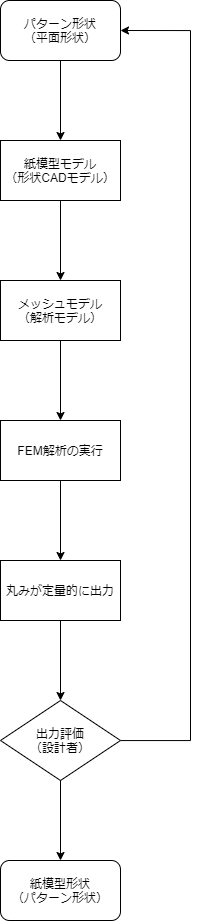
\includegraphics[scale=0.5]{./figure/caseA.png}
				\caption{システムフロチャート2}
			\end{figure}
			
	%\section{ガウス過程について}
ある入力パラメータ$ \bd{x} $と,出力パラメータ$ \bd{y} $が,正規分布$ N(\bd{\mu},\bd{\Sigma}) $に従うとき,出力がガウス過程に従うという.このガウス過程は,ニューラルネットワークの中間ノード数無限の極限としても知られる(Neal,1996).
	\subsection{ガウス過程の概要}
		入力パラメータ$ \bd{x} $と,出力パラメータ$ \bd{y} $について,その関係$ \bd{y} = \bd{f}(\bd{x})$を求めることを考える.単純な手法としては,以下のように,基底関数$ \bd{\Phi}(\bd{x}) $を用いて,以下のような重み付きの線形和で表し,この重みを最小二乗法などで求める手法である.
		\begin{equation}\label{eq:Ritz_ppoi}
			\bd{y} = \bd{\Phi}\bd{w}
		\end{equation}
		この基底関数には,以下のような動径基底関数を用いればよいとされ,この方法は,動径基底関数回帰と呼ばれる.
		\begin{equation}\label{eq:phieq}
			\phi_i = \{\bd{\Phi}\}_i = \exp\left(-\frac{(x-\mu_h)^2}{\sigma^2}\right)
		\end{equation}
		しかし,この手法は$ \mu_h $を,入力の定義域上になるべく多く配置させる必要があり,$ \bd{x} $の次元に対して指数的に増加する\footnote{次元の呪いとも呼ばれる}ため,現実的に解くのは非常に難しいとされる.
		
		そこで,$ \bd{w} $があるガウス分布$ N(0,\lambda^2\bd{I}) $に従うとするときについて考える.このとき,$ \bd{y} = \bd{\Phi}\bd{w} $もまた,ガウス分布に従う.このとき,モデルの期待値および分散は以下のように求められる.
		\begin{eqnarray}\label{eq:VarandAvg}
			E[\bd{y}] &=& E[\bd{\Phi}\bd{w}] = \bd{\Phi}E[\bd{w}]=0\\
			\Sigma &=& E[\bd{y}\bd{y}^T]-	E[\bd{y}]E[\bd{y}^T] = \lambda^2\bd{\Phi}\bd{\Phi}^T
		\end{eqnarray}
		よって,$ \bd{y} $はガウス分布$ N(\bd{0},\lambda^2\bd{\Phi}\bd{\Phi}^T) $に従う.$ \bd{K} =  \lambda^2\bd{\Phi}\bd{\Phi}^T$と置けば,$ \bd{K} $が求めれば,$ \bd{y} $のガウス分布を求めることができる.
		この$ \bd{K} $は,グラム行列,またはカーネル行列と呼ばれ,その行列が下記の条件を満たすように設計されなければならない.
		\begin{itemize}
			\item 逆行列の存在を保証する.
			\item 正定値を持つ.
			\item 固有値が全て正である
		\end{itemize}
		カーネル行列の各成分を示すカーネル関数として代表的なものは,以下で示すRBFがある.なお,$ \bd{\theta} = [\theta_1,\theta_2] $は,ハイパーパラメータと呼ばれる.
		\begin{equation}\label{eq:Kernel}
			k(\bd{x}_i,\bd{x}_j) = \theta_1 \exp\left(- \frac{|\bd{x}_i-\bd{x}_j|^2}{2 \theta_2^2}\right)
		\end{equation}
		このモデルを用いて,ある事前学習パラメータ$ \bd{X}=[\bd{x}_1,\bd{x}_2,\cdots,\bd{x}_n] $に対し,$ \bd{Y}=[y_1,y_2,\cdots,y_n] $という出力が得られている場合において,ある入力パラメータ$ \bd{x}_* $に対する$ y_* $は事後確率の期待値として表される.
		\begin{equation}
			y_* = \bd{k}_* \bd{K}^{-1} \bd{Y}
		\end{equation}
		ただし,$ \bd{k}_* = \{k(\bd{x}_*,\bd{x}_i)\}_{i=1}^{n} $である.
		
		ハイパーパラメータの定め方について述べる.このとき,確率関数の対数をとった尤度関数は以下のように表される.
		\begin{equation}\label{eq:Suudo}
			\log(p) = -\log|\bd{K}_{\theta}| - \bd{y}^T \bd{K}_{\theta}^{-1} \bd{y}+C
		\end{equation}
		ただし,ハイパーパラメータに無関係な定数をまとめて$ C $とおいている.一般にはこの尤度関数を最大化するような最適化問題を解くことによって,パラメータを得る.この最適化問題は解析的に微分を求めることができるため,勾配法を用いて解くケースが多い.
	\subsection{クラスタリングについて}
		出力として二値的な値を取る場合,出力の値を近似的に$ y = \sigma(\bd{x}) $と表す,ただし,$ \sigma(\bd{x}) $はシグモイド関数である.このとき,事後確率の出力は少し複雑となり,以下のように表される.
		\begin{equation}\label{eq:y_*=1}
			q = \Psi\left( \frac{\bd{k}_*^T \tilde{\bd{K}}^{-1} \tilde{\bd{\mu}}}{\sqrt{1+k(\bd{x}_*,\bd{x}_*)-\bd{k}_*^T \tilde{\bd{K}}^{-1} \bd{k}_*}} \right)
		\end{equation}
		ここで,$ \Psi $は累積分布関数を表す.また,$ \tilde{\bd{K}} $や$ \tilde{\bd{\mu}} $は特定のアルゴリズムを用いて求められる(事後学習のデータを用いることなく)が,ここでは省略する.
	\subsection{ベイズ最適化について}
	ベイズ最適化は,ガウス過程を応用する形になっており,ある目的関数$ f(\bd{x}) $を最小化するような$ \bd{x} $を求める手法である.ここでは,ある学習データが与えられる場合について考える(学習データがない場合は,一様に初期解を生成する手法があるらしい?).このとき,この最適化問題は,事後学習における平均および分散の関数で定める適当な関数の最適化問題に変換でき,関数を明示的に与える必要がないのが,ベイズ最適化の特徴である.この目的関数の定め方は色々あるが,ポピュラーなものとしてはEIがある.
	\begin{equation}\label{eq:Zeq}
		Z = \frac{\mu - f^+ -\xi}{\sigma}
	\end{equation}
	\begin{equation}
		a_{EI} = (\mu - f^+ -\xi)\Psi(Z) + \sigma \psi(Z)
	\end{equation}
	ただし,$ \psi(x) \sim N(0,1)$の正規分布関数である.
	\newpage
\vspace{10cm}
%%%%%%%%%%%%%%%%%%%%%%%%%%%%%%%%%%%%%%
% 3.達成できなかったこととその問題点
	%\articleSPRthree
%%%%%%%%%%%%%%%%%%%%%%%%%%%%%%%%%%%%%%

\vspace{14cm}
%%%%%%%%%%%%%%%%%%%%%%%%%%%%%%%%%%%%%%
	\articleSPRfour
	\articleSPRfive
\end{document}
